\section{BMS Software}

%\subsection{Design}
The BMS software is programmed on the Digital Unit. The purpose of the BMS software is to continually collect data from the Analog Front End and then inspect this data to see if the batteries are working as expected. Data is at least collected every second. However, if the collected data has parameters close to their respective thresholds then data collection increases to being done every 200 milliseconds. At this point a safety check of the parameters is executed - See BMS 2013 Documentation \cite{BMSDocumentation} (section 3.2.3).

This is done because it is assumed that if the data is far away from the thresholds, then they are most likely not exceeded as quick as if the data was close to the thresholds. It is very important to have a safe operating system with many safety checks, but it is also important to do as few calculations as possible. The reasoning for this is that the system should be in the power saving “sleep mode” as much as possible to save energy and thereby be as energy efficient as possible.

If the battery cells at startup has a voltage too high, the BMS system sets the cells to balance down in voltage with the help of bleeder resistors and sets the initiation of the system on a hold for four seconds. This gives the cells time to discharge. The twelve cells are also analyzed every second, so that if any threshold is exceeded, the Isolation Switch is opened, and will stay this way until the cells are balanced back within acceptable thresholds. This balancing is possible when a charger is connected. Lastly every second the collected data is sent via CAN-communication. After 20 seconds have passed, a State Of Charge analysis (SOC-analysis) is executed, this data is of course also sent via CAN-communication.

Details about how the software works can be found in the documentation of the BMS2013 \cite{BMSDocumentation} (section 3.2). Where the software is well documented with flowcharts, application models/class diagrams, function descriptions and code examples. It would be pointless to redocument the many functions, but the few changes made in 2014 is yet to be documented, which will be the focus of this documentation.
The BMS software consists of the following c- and h-files:\\
\begin{figure}[H]
	\centering
	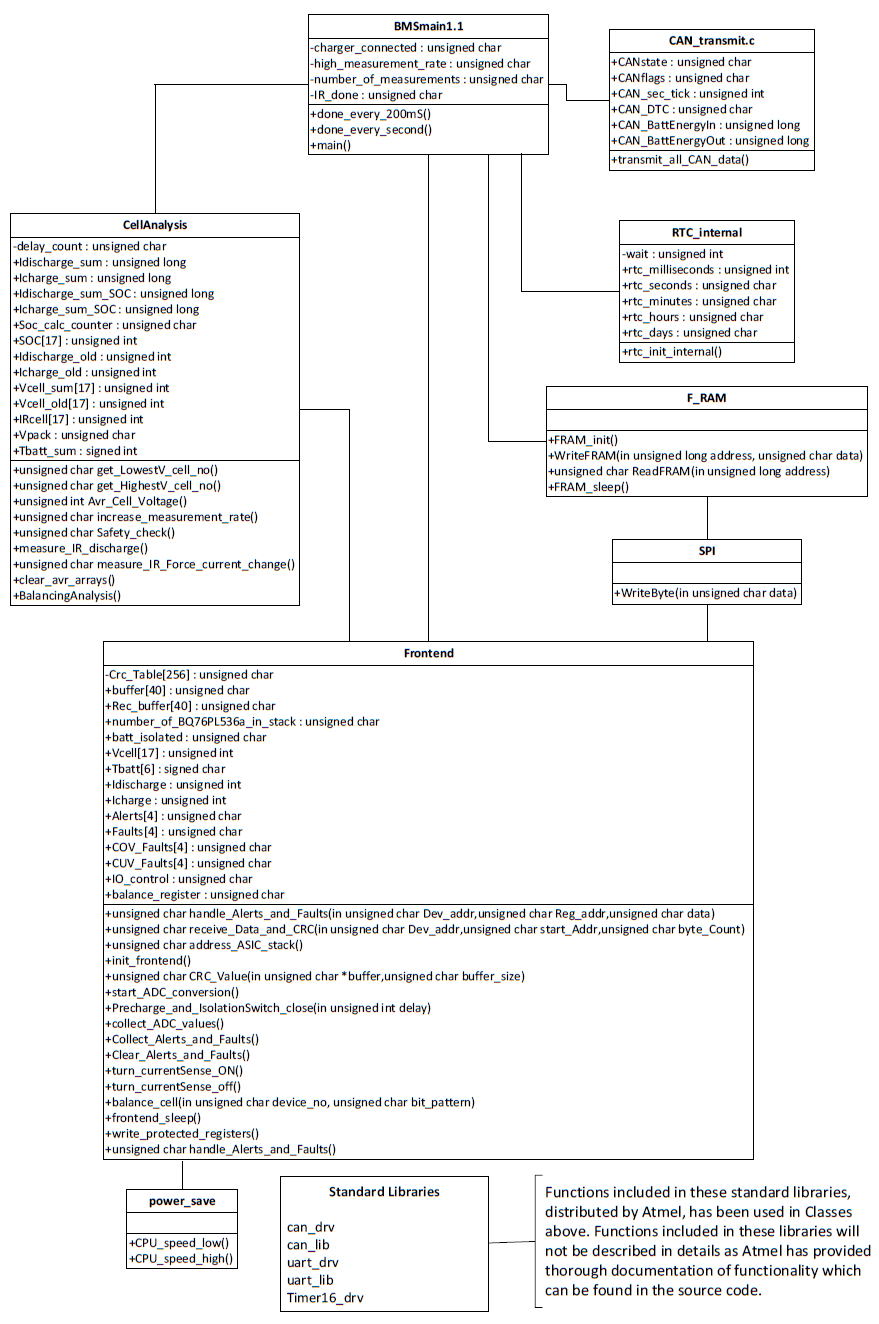
\includegraphics[width=1.0\linewidth]{Software/BMS-ClassDiagram.PNG}
	\caption{Class Diagram from 2013 BMS Documentation \cite{BMSDocumentation} (section 3.2.2).}
	\label{fig:SOFTWARE_BMS}
\end{figure}
The only function description that isn’t documented is the “CalculateSOC()” function. This is because “CalculateSOC()” was re-implemented as a function in 2014 instead of just being part of the “done\_every\_second()” function. Therefore the function description for the “CalculateSOC()” will be presented now. This function is located in the CellAnalysis.c file:
\begin{table}[h!]
	\centering
	\label{CalculateSOCfunction}
	\begin{tabular}{|p{4 cm}|p{9 cm}|}
		\hline
		\textbf{Function:} & \textbf{void CalculateSOC(void)}	\\\hline
		Parameters	& None	\\\hline
		Return Value	& None	\\\hline
		Description of function	& After data has been collected this function can be called and the state of charge will be found by compared the value of the cell voltages and ten different levels of voltage. This way the state of charge will be represented from 1 to 10, where 1 is 10 percent and 10 is 100 percent \fxnote{JENS - når koden virkede fik vi SOC udskrifter der var omkring 40-45 med det halvt opladede batteri - Så forstår ikke hvorfor værdien går fra 1-10}.	\\\hline
	\end{tabular}
	\caption{function description of the CalculateSOC function}
\end{table}

The rest of the changes made from 2013 to 2014 that are worth mentioning are the following definitions:\\
\begin{table}[h!]
	\centering
	\label{changedDefines}
	\begin{tabular}{|p{4 cm}|p{4 cm}|p{4 cm}|}
		\hline
		\textbf{definition} & \textbf{value after (2014)}	& \textbf{value before (2013)}	\\\hline
		Cell\_count	& 12	& 6	\\\hline
		AFE\_count	& 2	& 1	\\\hline
		capacity	& 2200	& 3300	\\\hline
		Icharge\_max	& 8000	& 15000	\\\hline
		Idischarge\_max	& 25000	& 55000	\\\hline
	\end{tabular}
	\caption{Overview of the changes since 2013}
\end{table}

This is some of the changes that seemingly happened in 2014 without being documented. The most important change that was made in 2014 is not revealed yet though. This change is the addition of the addresses to the Analog Front End Extension Module that was added in 2014 for measuring the second battery's voltage levels:\\
\begin{figure}[H]
	\centering
	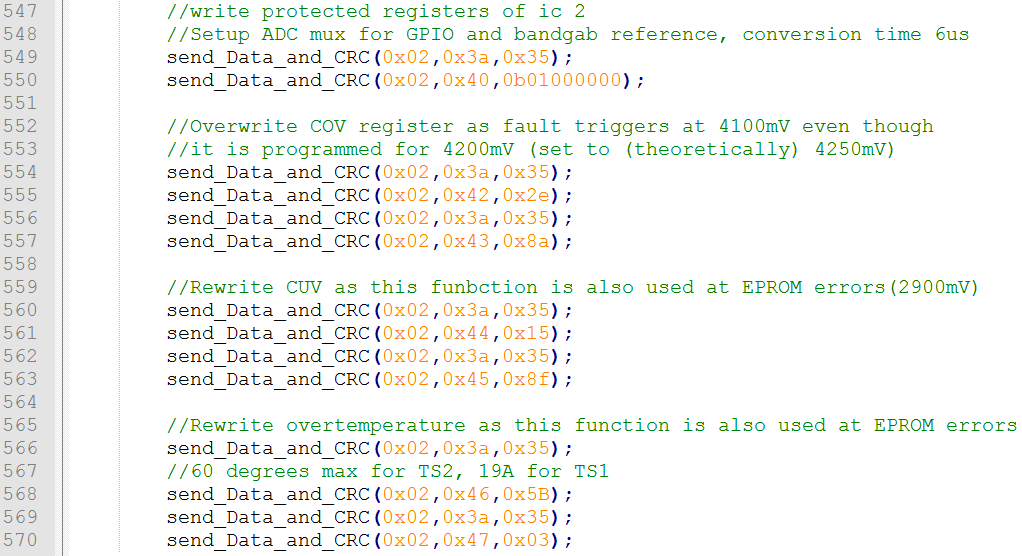
\includegraphics[width=1.0\linewidth]{Software/AddressAdditionsBMS.PNG}
	\caption{Address additions to the Analog Front End Extension Module}
	\label{fig:AddressAdditions_BMS}
\end{figure}

This is what makes it possible to read from the additional Analog Front End Extension Module and thereby makes it possible to analyze two batteries at the same time.

%\subsection{Implementation}


\subsection{Unit test}
When it was discovered that the software from SEM2014 was on the Digital Unit a test was made to ensure that the software worked as promised. This test was made by connecting the micro-USB connector on the Analog Front End to the USB port on a PC. Thereafter by using Tera Term, the information from the batteries' cells were requested from the Digital Unit, read by the Analog Front End and printed to Tera Term.\\ 
This test was a success, because all the cells had voltages around 3.8 V, which is within the thresholds from 3 V to 4.2 V. The temperature was also registered correctly at 25 degrees celsius, which also was as expected since the batteries did not have any strong load on them such as the motor.\\
A picture of the test can be seen on the following figure:\\
\begin{figure}[H]
	\centering
	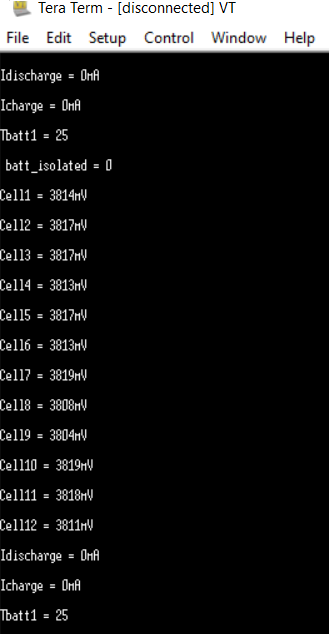
\includegraphics[width=0.5\linewidth]{Software/BMS_teraterm_test.PNG}
	\caption{Test of the software to BMS}
	\label{fig:SoftwareTest_teraterm_BMS}
\end{figure}

Now only the CAN-communication is needed to be tested. For testing the CAN-communication the corresponding requirement in the 2013 BMS documentation accept test was executed (BMS\_F.8) \cite{BMSDocumentation} (section 4.2.2).\\

After installing PCAN-view the CAN/USB converter (PCAN-USB from Peak-System) was connected from the OLIMEX AVR-CAN development board to a PC. PCAN-view did not receive any information from the CAN-communication. To be sure Analog Discovery was used on the CAN connector to see if anything was sent out. WaveForms' Digital Logic Analyzer was used after the CANL, CANH, VIN and GND pins were connected to Analog Discovery:\\
\begin{figure}[H]
	\centering
	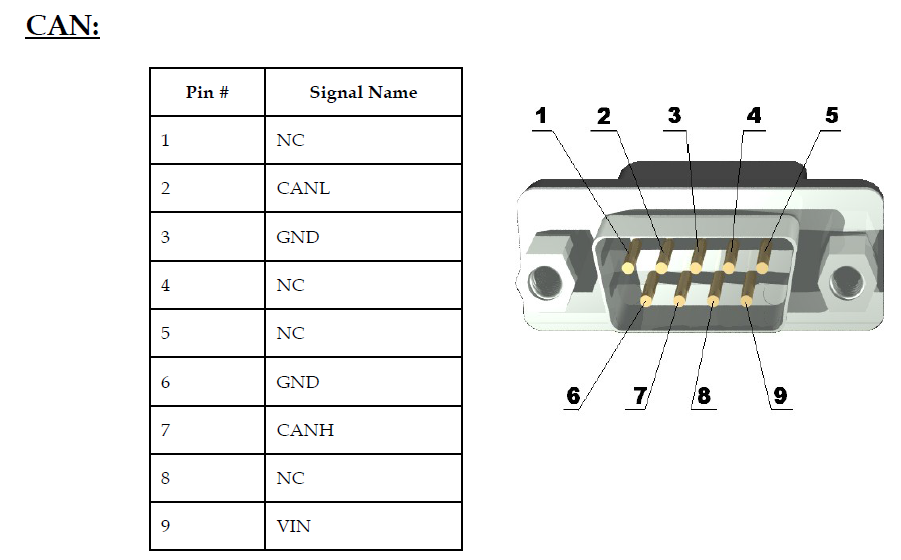
\includegraphics[width=0.5\linewidth]{Software/SnipFromOlimexDatasheet.PNG}
	\caption{Excerpt from OLIMEX AVR-CAN development board datasheet \cite{BMSAVRCAN}.}
	\label{fig:OLIMEX_AVR-CAN_BMS}
\end{figure}

The result was that nothing other than noise was received from the CAN bus.
From the documentation of BMS 2013 \cite{BMSDocumentation} that Jonas Nyborg made, the CAN-communication was documented and claimed to be already tested and well functioning.\\
The reason for why the CAN-communication not operating as expected was therefore an important question to be answered. The CAN-communication software was then inspected to see if we could find the reason for it not operating correctly. No mistakes were to be found, which let the group to the idea that that maybe Jonas Nyborg had commented out the "transmit\_all\_CAN\_data();" in the "done\_every\_second()" function. Contact was made with Jonas Nyborg and the idea was confirmed to be the case, because the team at Rotterdam SEM2014 did not need the CAN-communication hence power could be saved.\\
After knowing the CAN-communication was not programmed properly to the Digital Unit, the software was reprogrammed to the Digital Unit. After this was done the BMS did only read from one of the batteries and it was discovered that the software that was available, was the 2013 software, that was not compatible with two batteries at once.\\
Contact was made with Jonas Nyborg yet again, but after a few days the BMS software that Nyborg sent was still outdated, with the words; "If anybody has the newest BMS software version saved, it would be AU Campus Herning and their SEM2014 dropbox". This was discussed with Carl Jakobsen and the day after this dropbox was declared non-existent.\\
Since the BMS software was not ready for SEM2016 and the BMS software for SEM2014 was not to be found, the group tried to rebuild the changes made in 2014, so that the BMS software also would work with multiple batteries operating at the same time. In this process the group learned a lot about the BMS software, but after many tries of programming and testing a wire from the Analog Front End Extension Module was connected wrongly to the Analog Front End, which resulted in the destruction of the "BQ76PL536A-Q1" \cite{BMSBattIC} on each board. This was also explained earlier in the BMS hardware section.\\
A few days after contact was made with Simon Møiniche Skov, a person who worked on the SEM2014 project. He was asked if he had the newest version of the BMS software. A meeting with him took place and the software version was received. This version was the one used in SEM2014, the one that was sought and the one that has been discussed earlier of which changes that were made to this version compared to the well documented SEM2013 version.\\
Since the software version that was tested earlier and is now found and secured, the software should be ready for use, but the CAN-communication could not be tested before the Analog Front End and Analog Front End Extension Module could be fixed.\\  